%\documentclass[useAMS, usenatbib,usegraphicx,letter]{mn2e}
%\documentclass[11pt]{article}
\documentclass[reprint,aps,prd,superscriptaddress,showkeys,showpacs]{revtex4-1}
\usepackage{epsfig,amsmath,natbib}

\usepackage{aas_macros}
\usepackage{amssymb}
\usepackage{amsmath}
\usepackage{dsfont}
\usepackage{hyperref}
\usepackage{color}
\usepackage{pbox}
\usepackage{booktabs}

\hypersetup{
	colorlinks=false,
	citecolor=green
}
% \usepackage{graphicx}
% \usepackage{epstopdf}
% \usepackage{natbib}

%%%%%%%%%%%%%%%%%
%Custom commands%
%%%%%%%%%%%%%%%%%

\newcommand{\bb}[1]{\mathbf{#1}}
\newcommand{\bbh}[1]{\mathbf{\hat{#1}}}
\newcommand{\h}[1]{\hat{#1}}
\newcommand{\ttt}[1]{\texttt{#1}}
\newcommand{\LT}{\texttt{LensTools} }

%%%%%%%%%%%%%%%%%%%%%%%%%%%%%%%%%%%%%%%%%%%%%%

\begin{document}

\title{Mocking the Weak Lensing universe: the LensTools computing package}

\author{Andrea Petri}
\email{apetri@phys.columbia.edu}
\affiliation{Department of Physics, Columbia University, New York, NY 10027, USA}
\affiliation{Physics Department, Brookhaven National Laboratory, Upton, NY 11973, USA}

\date{\today}

\label{firstpage}

\begin{abstract}
We present a newly developed software package which implements a wide range of routines frequently used in Weak Gravitational Lensing (WL). With the continuously increasing size of the WL scientific community we feel that easy to use APIs for common calculations are a necessity to ensure efficiency and coordination across different working groups. Coupled with existing open source codes, such as \ttt{CAMB}\citep{CAMB} and \ttt{GADGET2}\citep{Gadget2}, \LT brings together a fully functional cosmic shear simulation pipeline which, complemented with a variety of WL feature measurement tools and parameter sampling routines, provides easy access to the numerics for theoretical studies of WL as well as for experiment forecasts. Being implemented in \ttt{python}\citep{python}, \LT takes full advantage of a range of state--of--the art techniques developed by the large and growing open--source software community \citep{scipy,pandas,astropy}.    
    
\end{abstract}


\keywords{Weak Gravitational Lensing --- Simulations}
\pacs{98.80.-k, 95.36.+x, 95.30.Sf, 98.62.Sb}

\maketitle


%%%%%%%%%%%%%%%%%%%%%%%%%% INTRO %%%%%%%%%%%%%%%%%%%%%%%%%%%%%%%%%%%%%%%%%%%%%%%%%%%%%%%%

\section{Introduction}
%
Cosmology is entering a new, data driven era. After the Cosmic Microwave Background (CMB) \citep{WMAP,PlanckXVI2013} provided strong experimental evidences of cosmological theories, a variety of different probes have been proposed to unveil the secret of the cosmos. Weak Gravitational Lensing uses the correlation between image distortions of background sources by Large Scale Structure (LSS) to infer cosmological parameters \citep{WLprimer}. Because WL probes are sensitive to the late universe, where the density fluctuations are in the non--linear regime, the cosmological information might not be all contained in quadratic features such as two--point correlation functions. In the theoretical study of more complicated WL features (see for example \citep{3pcf1,bispectrum1,moments1,peaks1} for a non comprehensive list), simulation pipelines play a vital role as in general these features cannot be predicted analitically from the cosmological parameters. In this work we present a flexible, customizable and easy to deploy WL simulation pipeline that bridegs the gap between simulations of shear fields, feature measurement from simulated images and cosmological parameter estimation. The paper is organized as follows: first we give an overview of the code structure, highlight the core routines and present the benchmarks and complexity of the expensive computing steps. We complement the work with some illustrative examples on how to use \LT for some of the former tasks. We finally discuss the future prospects of the software development.     

%%%%%%%%%%%%%%%%%%% Shear simulations %%%%%%%%%%%%%%%%%%%%%%%%%%%%%%%%%%%%%%%

\section{Shear simulations} 

\subsection{Formalism}
%
In this paragraph we give an overview of the \LT shear field simulation pipeline. This is a series of routines that, broadly speaking, take a vector of cosmological parameters $\bb{p}$ and some resolution parameters to produce random realizations of shear fields $\pmb{\gamma}(\pmb{\theta})$ in that particular cosmology ($\pmb{\theta}=(\theta_x,\theta_y)$ is the angle on sky as seen from the observer). Given a background source at redshift $z_s$, the matter density fluctuations $\delta(\bb{x},z)$ in between the observer and the source will cause its apparent shape to be distorted; the cosmic shear $\pmb{\gamma}$ is a measurement of the apparent source ellipticity, assuming the unperturbed shape is a circle. The multi--lens--plane algorithm \citep{RayTracingHartlap} is a popular techique to compute light ray deflections across the path $z\in[z_s,0]$ and hence to compute the apparent source shape distortion. The mass distribution between the source and the observer is approximated as a sequence of two dimensional lenses perpendicular to the line of sight, of thickness $\Delta$ and a surface density $\sigma$ given by 

\begin{equation}
\label{surfacedensity}
\sigma(\bb{x},z) = \frac{3H_0^2\Omega_m\chi(z)}{2c^2a(z)}\int_\Delta dz'\delta(\bb{x},z')
\end{equation}
%
Where $\chi$ is the lens comoving distance and $a=(1/1+z)$ the scale factor. A light ray crossing a lens at redshift $z$ at a transverse position $\bb{x}$ will be deflected by a small angle $\pmb{\alpha}$ which can be shown to be the gradient of the 2D gravitational potential $\phi$ (see again \citep{RayTracingHartlap}) 
%
\begin{equation}
\label{poisson}
\begin{matrix}
& \nabla^2_\bb{x} \phi(\bb{x},z) = 2\sigma(\bb{x},z) \\ \\
& \pmb{\alpha}(\bb{x},z) = \nabla_\bb{x} \phi(\bb{x},z) \\ \\
& \bb{T}(\bb{x},z) = \nabla_\bb{x}\nabla_\bb{x}^T \phi(\bb{x},z)
\end{matrix}
\end{equation}
%
where we indicated $\bb{T}$ as the gradient of the deflection, which will be called \textit{shear tensor} throughout the rest of the paper. The trajectory of a light ray $\bb{x}(z)$ follows the geodesic equation

\begin{equation}
\label{geodesic3D}
\frac{d^2\bb{x}}{d\chi^2} = -\frac{2}{c^2}\nabla_\bb{x_\perp}\Phi(\bb{x},z)
\end{equation}
%
which can be translated into a second order differential equation for the light ray angular position $\pmb{\beta}(z)=\bb{x}_\perp(z)/\chi(z)$ as seen from the observer. Following \citep{RayTracingHartlap}, the trajectory of each light ray originating at $\pmb{\beta}(0)=\pmb{\theta}$ can be calculated solving numerically a discretized version of (\ref{geodesic3D}), assuming a finite number of lenses placed at a finite number of redshifts $\{z_k\}$:
%

\begin{widetext}

\begin{equation}
\label{geodesic2D}
\pmb{\beta}_{k} = \sum_{i=1}^k\delta\pmb{\beta}_i 
\end{equation}

\begin{equation}
\delta\pmb{\beta}_k = (A_k-1)\delta\pmb{\beta}_{k-1} + C_k\pmb{\alpha}_k 
\end{equation}

\begin{equation}
\bb{U}_{k} = \sum_{i=1}^k\delta\bb{U}_i 
\end{equation}

\begin{equation}
\delta\bb{U}_k = (A_k-1)\delta\bb{U}_{k-1} + C_k\bb{T}_k\bb{U}_k
\end{equation}

\end{widetext}
%
where $\bb{U}$ is the jacobian matrix of the trajectory $\pmb{\beta}$ with respect to the initial light ray position $\pmb{\theta}$, $\bb{U}_k=\nabla_{\pmb{\theta}}\pmb{\beta}_k(\pmb{\theta})$. The factors $A_k,C_k$ depend on the geometry of the lens system

\begin{widetext}

\begin{equation}
A_k = \frac{\chi_{k+1}}{\chi_{k+2}}\left(1 + \frac{\chi_{k+2}-\chi_{k+1}}{\chi_{k+1}-\chi_k}\right) \,\,\,\, ; \,\,\,\, C_k = \frac{\chi_{k+1}}{\chi_{k+2}} - 1 \\ \\
\end{equation} 

\end{widetext}

%
where we use the subscript $k$ to indicate the redshift $z_k$ of the $k$--th lens for notational simplicity. After tracing the evolution of $\bb{U}$ from the observer to the source at $z_s$, we are able to evaluate the cosmic shear $\pmb{\gamma}$ and convergence $\kappa$ at $z_s$ looking at the components of $\bb{U}$
\begin{equation}
\bb{U}(\pmb{\theta},z_s) = (1-\kappa(\pmb{\theta}))\mathds{1}_{2\times2} - \gamma^1(\pmb{\theta})\sigma^3 - \gamma^2(\pmb{\theta})\sigma^1
\end{equation}
%
where we indicated $\mathds{1}_{2\times2}$ as the identity matrix and $\sigma^{1,3}$ as the first and third Pauli matrices. The iterative solution of (\ref{geodesic2D}) requires the knowledge of the density fluctuation $\delta(\bb{x},z)$, from which the lens surface density $\sigma$ and gravitational potential $\phi$ can be inferred. $\delta$ can be calculated running $N$--body simulations, in which the matter distribution in the universe is approximated as a set of $N_p$ particles of mass $M_p$, which evolve gravitationally. For this purpose we use the publicly available code \ttt{GADGET2}\citep{Gadget2}, although alternatives can be adopted (see \citep{HACC} for example). Once the $N$--body simulations are ran, \LT provides a \ttt{python} implementation of the multi--lens--plane algorithm \citep{RayTracingHartlap} described above, which takes care of projecting the density fluctuation on two dimensional lenses as in (\ref{surfacedensity}), solving the Poisson equation as in (\ref{poisson}), and computing the light ray deflections as in (\ref{geodesic2D}). 

\subsection{Code}
%

\subsection{Performance}
%
Table \ref{benchmarktable} shows a summary of the ray--tracing operations performed by \LT, indicating the complexity and runtime of each operation for a selected test case.  

\begin{table*}
\begin{tabular}{l|c|c|c}
\toprule
{Step} &            Complexity &            Test case &           Runtime \\ \hline \hline
\midrule
\multicolumn{4}{c}{\textbf{Lens generation}} \\ \hline
Snapshot input & $O(N_p/N_t)$  & $N_p=512^3$, $N_t=16$  &  \\
Gridding        & $O(N_p/N_t)$   & $N_p=512^3$, $N_t=16$  &  \\
MPI Communication  & $O(L_p\log{N_t})$   & $N_t=16$, $L_p=4096^2$  &   \\
Poisson solver           & $O(L_p\log{L_p})$ & $L_p=4096^2$  &      \\
Lens output           & $O(L_p)$ & $L_p=4096^2$   &   \\ \hline \hline

\multicolumn{4}{c}{\textbf{Ray tracing}} \\ \hline
Lens input &  $O(L_p)$ & $L_p=4096^2$ &  \\
Random lens shift &  $O(L_p)$ & $L_p=4096^2$ &  \\
Deflection calculation        &  $O(N_r)$ & $N_r=2048^2$   &  \\
Shear tensor product               &  $O(N_r)$ & $N_r=2048^2$   &   \\ \hline \hline

\bottomrule
\end{tabular}
\caption{Summary of the ray--tracing benchmarks: each $N$--body snapshot is divided in $N_t$ files, which are read in parallel and contain a total of $N_p$ particles. After the gridding procedure (\ref{surfacedensity}) is performed by each task, the total sufrace density (computed for a plane of $L_p$ pixels) is collected by the master task, which then proceeds in solving the Poission equation (\ref{poisson}) via Fast Fourier Transforms and saves the output to disk. In a subsequent step, the lens densities are read from disk, and the geodesic equations (\ref{geodesic2D}) are solved for $N_r$ different starting positions $\pmb{\theta}$ that allow to reconstruct the shear and convergence fields $\pmb{\gamma},\kappa$.}
\label{benchmarktable}
\end{table*}

\begin{figure*}
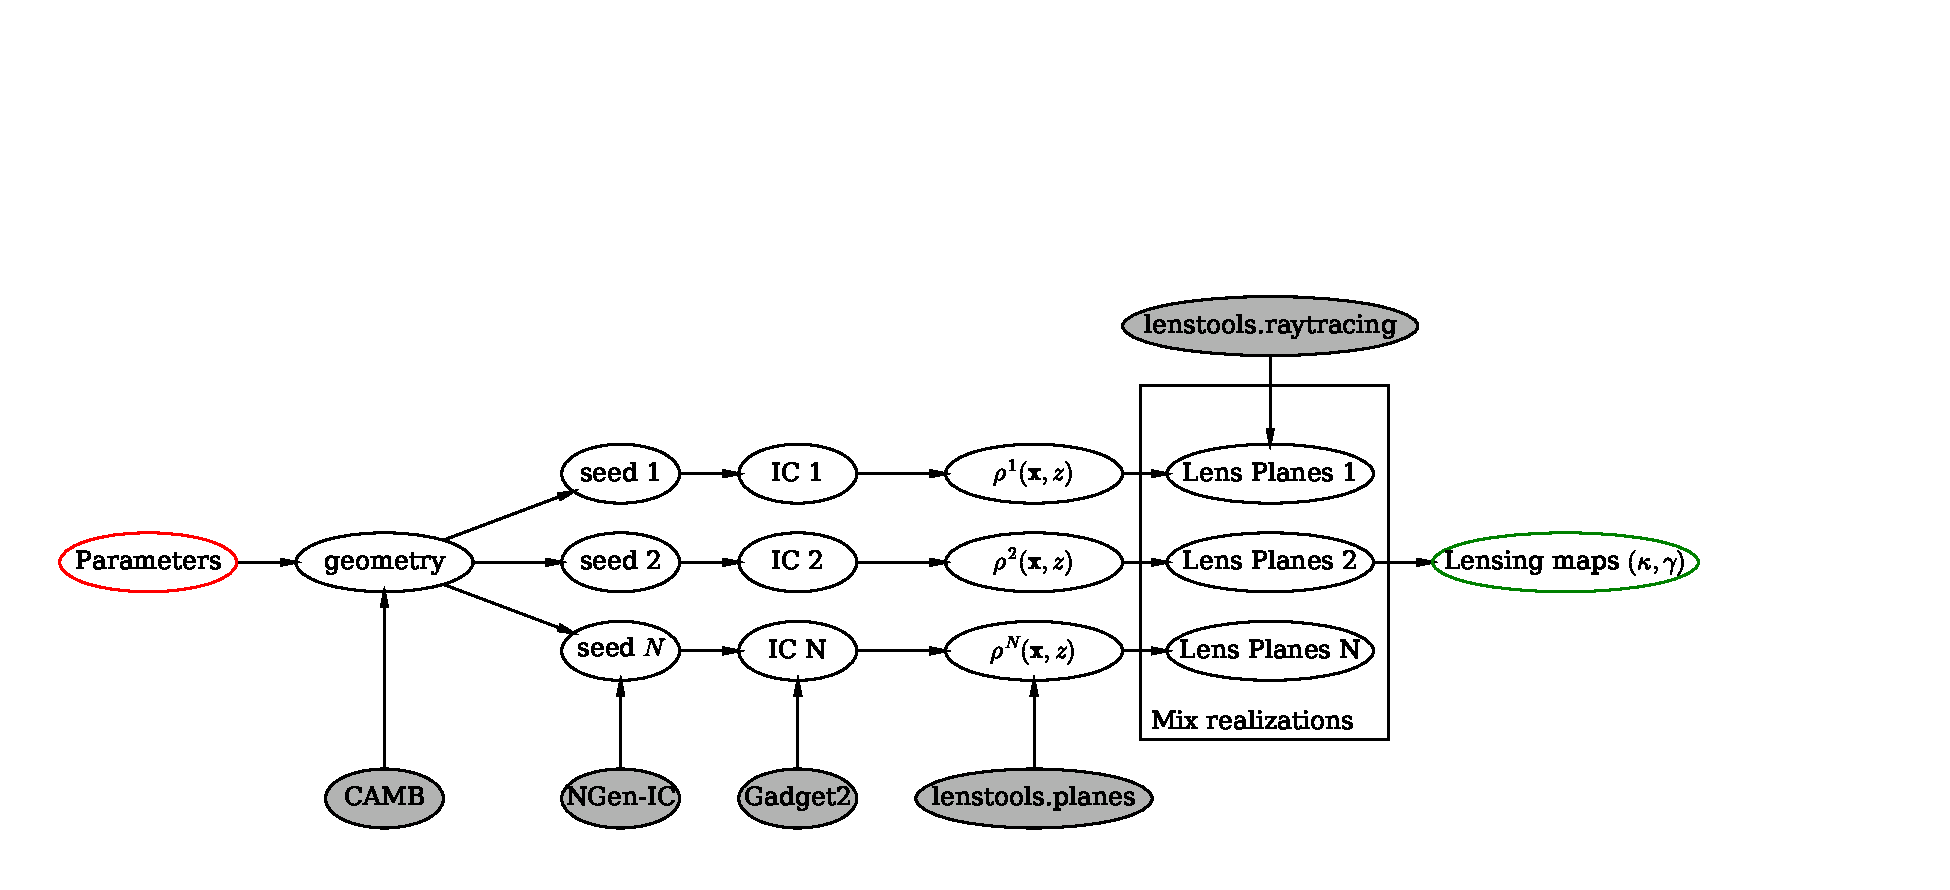
\includegraphics[scale=0.6]{Figures/flow.eps}
\caption{Schematic of the \LT WL shear simulation pipeline}
\label{pipescheme}
\end{figure*}

%%%%%%%%%%%%%%%%%%%%%%%%%%%%%%%%%%%%%%%%%%%%%%%%%%%%%%%%%%%%%%%%%%%%%%%%%%%%%%%%%%%%%%%%%%%%%%%%%%%%%%%%%%%%%%%%%%%%%%%%%%%%%%%%%%%%%%%%%%%%%

\section{Image analysis}

%%%%%%%%%%%%%%%%%%%%%%%%%%%%%%%%%%%%%%%%%%%%%%%%%%%%%%%%%%%%%%%%%%%%%%%%%%%%%%%%%%%%%%%%%%%%%%%%%%%%%%%%%%%%%%%%%%%%%%%%%%%%%%%%%%%%%%%%%%%%%

\section{Cosmology constraints}

\begin{figure}
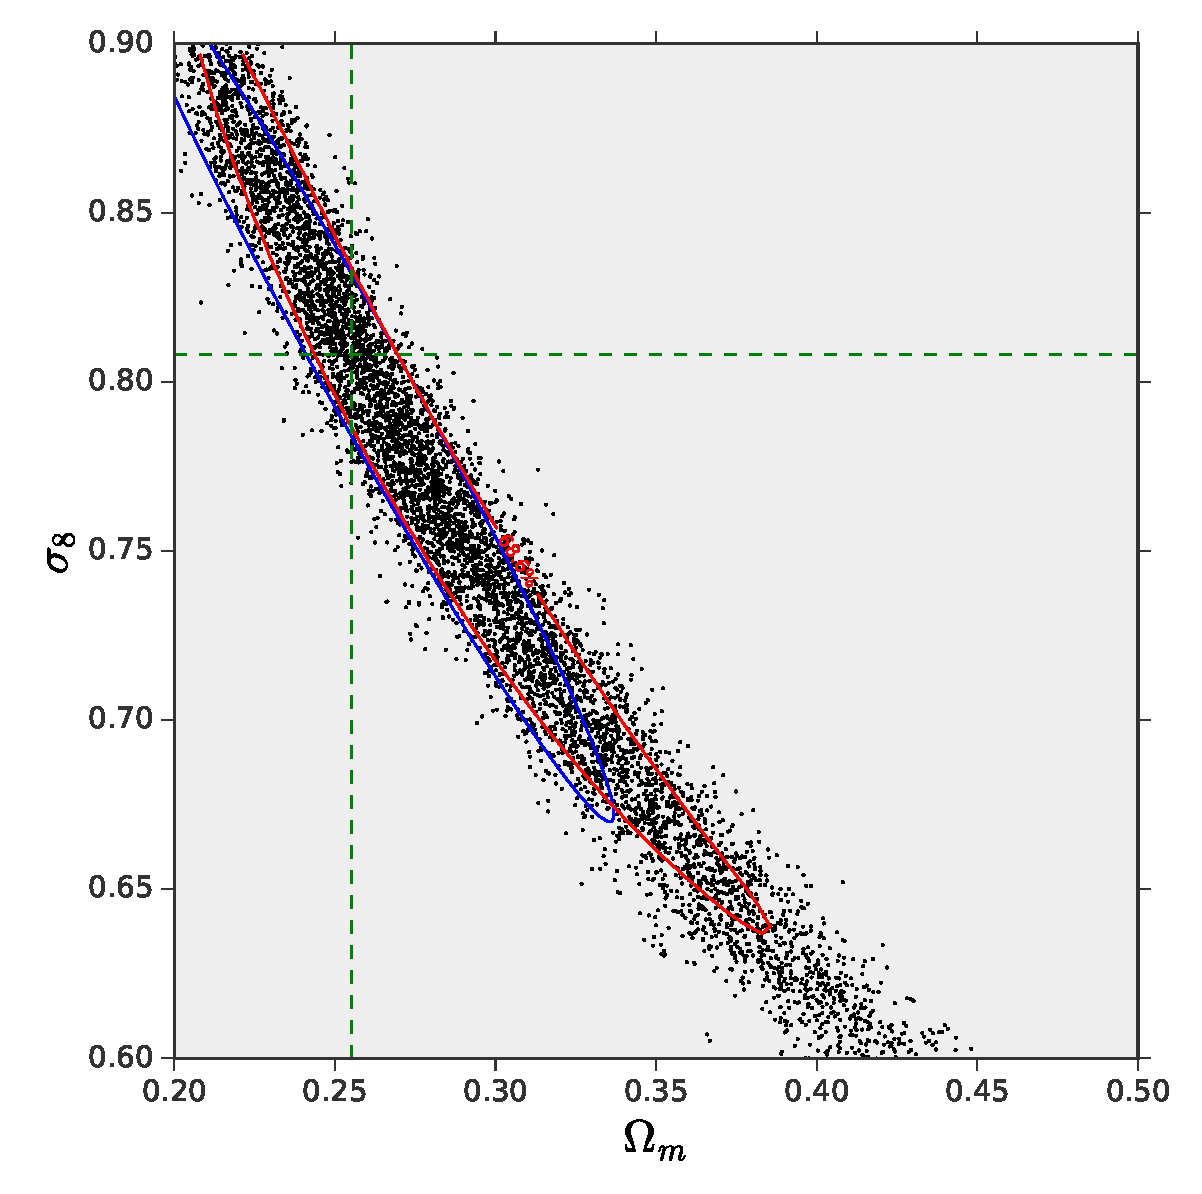
\includegraphics[scale=0.4]{Figures/parameter_sampling.eps}
\caption{Parameter sampling examples}
\label{samplingfig}
\end{figure}

%%%%%%%%%%%%%%%%%% FUTURE %%%%%%%%%%%%%%%%%%%%%%%%%%%%%%%%%%%%%

\section{Future developments}

%%%%%%%%%%%%%%%%%% CONCLUSION %%%%%%%%%%%%%%%%%%%%%%%%%%%%%%%%%%%%%

\section{Conclusion}

%%%%%%%%%%%%%%%%%%%%%%%%%% ACKNOWLEDGMENTS %%%%%%%%%%%%%%%%%%%%%%%%%%%%%%%%%%%%%%%%%%%%%%%%%%%%%%
 

\section*{Acknowledgements}


\bibliography{ref}
\label{lastpage}
\end{document}
